\section{Vergleich mit Gnu Scientific Library}

In diesem Abschnitt wollen wir die \naglib mit der {\it Gnu Scientific Library} (GSL) vergleichen.
Als Kriterien verwenden wir zum einen den gebotenen Funktionsumfang in den Bereichen Korrelation und Regression, als auch die Leistung der Funktionen.

% TODO: Kurze Einführung GSL 

\subsection{Funktionsumfang}
\label{sec:funktionsumfang}

% TODO: Hier kommt der Funktionsumfang für die Korrelation hin...

Auch im Bereich der Regression gibt es große Unterschiede in der Funktionalität.
Die in dieser Arbeit behandelten Regressionsarten finden sich aber in beiden Bibliotheken.
Während die einfache Regression in der \naglib von der Funktion nag\_simple\_linear\_regression berechnet wird, existieren in der GSL mehrere Funktionen zu diesem Zweck.
Diese sind gsl\_fit\_linear für eine Regression mit konstantem Term, gsl\_fit\_wlinear für gewichtete Beobachtungen, sowie gsl\_fit\_mul bzw. gsl\_fit\_wmul für Regressionen ohne konstanten Term.

Ähnlich verhält es sich mit der multiplen Regression.
Hier stehen den beiden NAG Funktionen nag\_regsn\_mult\_linear und nag\_regress\_confid\_interval (für Konfidenzintervalle) die Funktionen  gsl\_multifit\_linear, gsl\_multifit\_wlinear und gsl\_multifit\_linear\_residuals (Berechnung der Residuen) gegenüber.
Zusätzlich ist es bei Benutzung der GSL möglich mit den Funktionen gsl\_multifit\_linear\_svd und gsl\_multifit\_usvd Einfluss auf die Berechnung der Singulärwertzerlegung zu nehmen, welche in der GSL zur Berechnung der Koeffizienten verwendet wird.
Die Dokumentation aller GSL Funktionen zur Regression ist unter \cite{FreeSoftwareFoundation2011} verfügbar.
Damit ist die Funktionalität der GSL allerdings auch erschöpft, während in der \naglib noch weitere Funktionalität zur Verfügung steht.

Eine weitere Möglichkeit der \naglib ist es, vorhandene Berechnungen weiterzuverwenden.
Mit Funktionen wie nag\_regsn\_mult\_linear\_add\_var, nag\_regsn\_mult\_linear\_delete\_var oder nag\_regsn\_mult\_linear\_addrem\_obs können zum Beispiel Variablen oder Beobachtungen zum Modell hinzugefügt oder gelöscht werden.
Eine Aktualisierung der Koeffizienten erfolgt dann mit nag\_regsn\_mult\_linear\_upd\_model.
Es muss allerdings gesagt werden, dass diese Methode nicht immer zum gleichen Ergebnis führt wie die direkte Berechnung.
Stattdessen werden die bereits berechneten Koeffizienten nur minimal verändert und der neue Koeffizient wird so gewählt, dass die Residuen minimal sind. 
Außerdem werden auch Methoden angeboten, welche die Bestimmung des Regressionsmodells vereinfachen.
So berechnet die Funktion nag\_all\_regsn beispielsweise die Quadratsumme der Residuen aller möglichen Regressionen für eine Menge von unabhägigen Variablen.
Weiterhin ist es möglich andere Verteilungen als die Normalverteilung für die Fehlerterme anzunehmen (zB. nag\_glm\_binomial).
Zuletzt existieren hier auch Funktionen für spezialisiertere Regressionsarten, wie zum Beispiel die robuste Regression oder die Ridge-Regression.

\subsection{Leistungsanalyse}
\label{sec:leistungsanalyse}

% TODO: Cluster, Compiler (kurz)

% Graphik mit allen Kurven:
\begin{figure}[t]
  \centering
  \begin{narrow}{-0.2\textwidth}{0.2\textwidth}
    \subfloat[][Dauer der einfachen linearen Regression von NAG und GSL mit zunehmenden Beobachtungen aus dem Mietspiegeldatensatz\cite{Fahrmeir2011}.]{
      \label{fig:analysis:sim_reg_rent}
      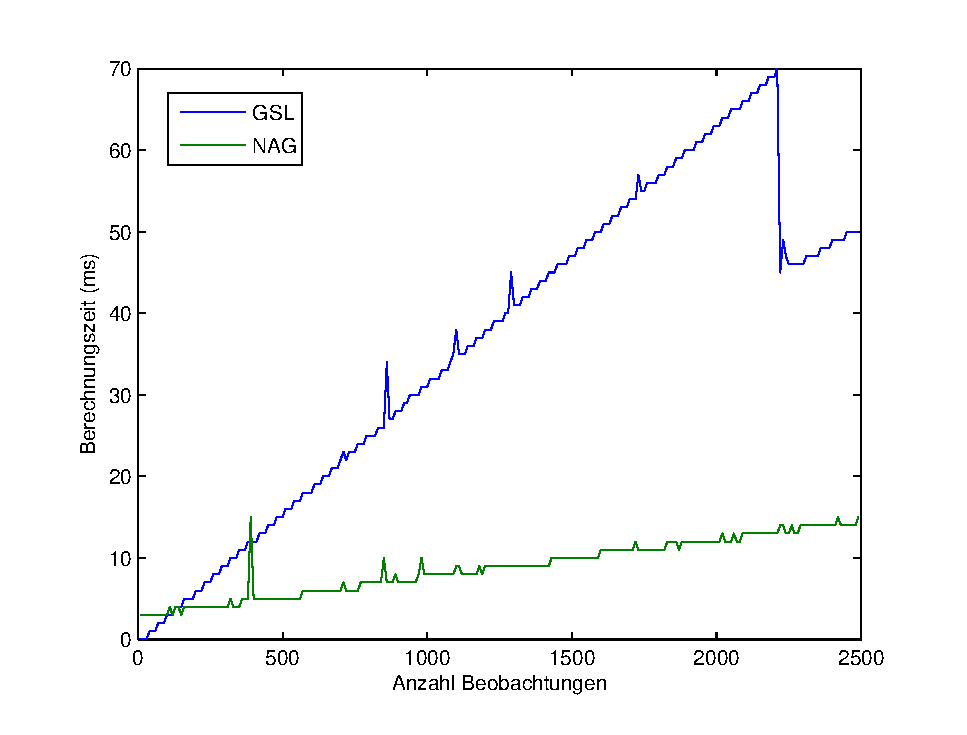
\includegraphics[width=0.6\textwidth]{figures/simple_reg_comp_rent}
    }
    \subfloat[][Dauer der einfachen linearen Regression von NAG und GSL mit zufälligen Daten.]{
      \label{fig:analysis:sim_reg_rand}
      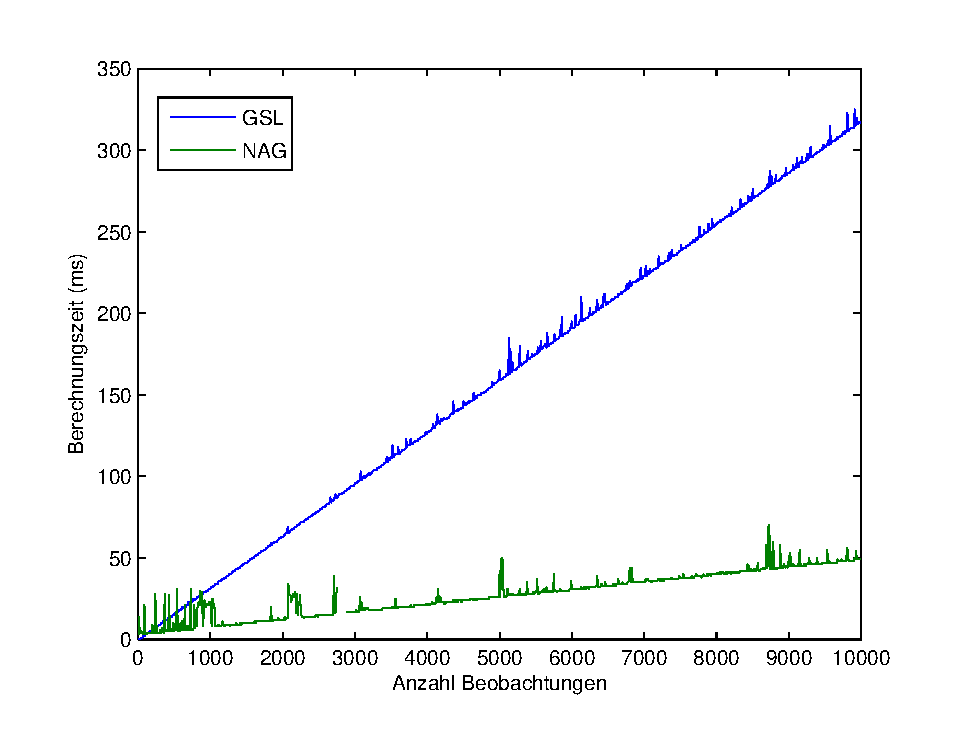
\includegraphics[width=0.6\textwidth]{figures/simple_reg_comp}
    }\\
    \subfloat[][Dauer der multiplen Regression von NAG und GSL mit 6 Merkmalen und zufälligen Daten.]{
      \label{fig:analysis:mul_reg_obs}
      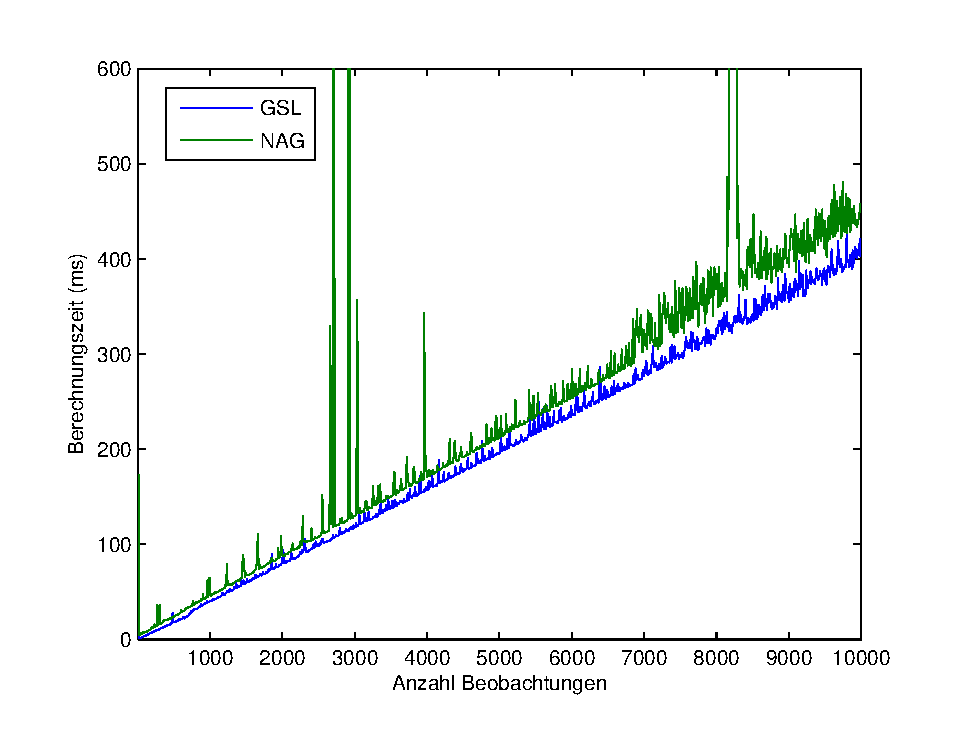
\includegraphics[width=0.6\textwidth]{figures/multi_reg_comp_6_var}
    }
    \subfloat[][Dauer der multiplen Regression von NAG und GSL mit 2500 Beobachtungen und zufälligen Daten.]{
      \label{fig:analysis:mul_reg_vars}
      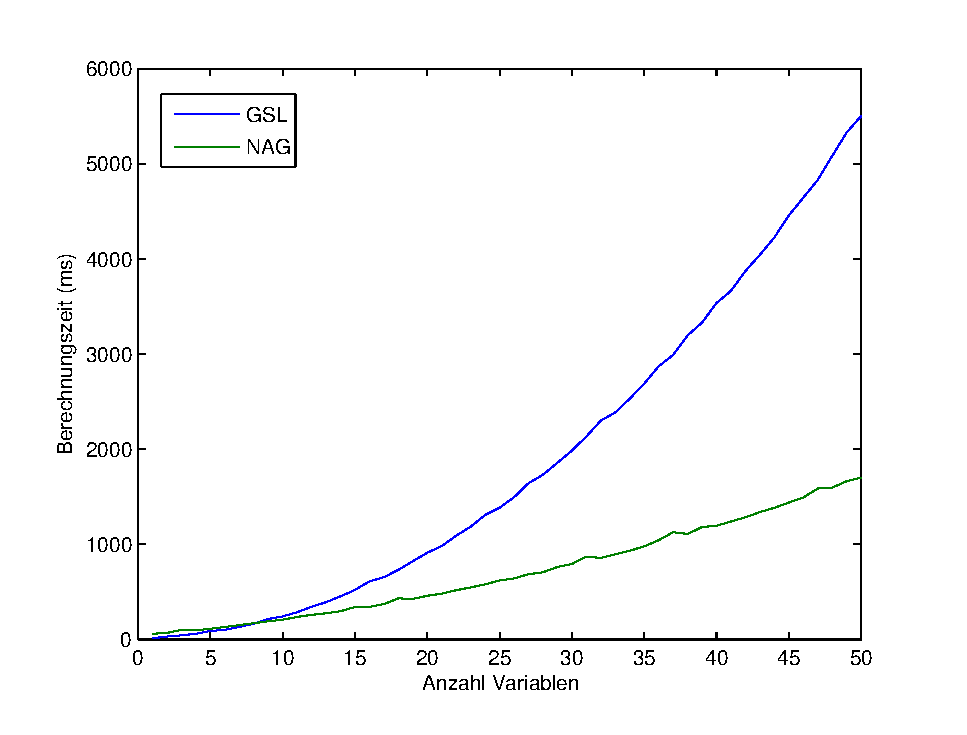
\includegraphics[width=0.6\textwidth]{figures/multi_reg_vars_2500_obs_rand}
    }\\
    \subfloat[][Unterschied zwischen direkter Berechnung und Aktualisierung mit Daten aus dem  Mietspiegeldatensatz\cite{Fahrmeir2011}.]{
      \label{fig:analysis:mul_reg_rent_act}
      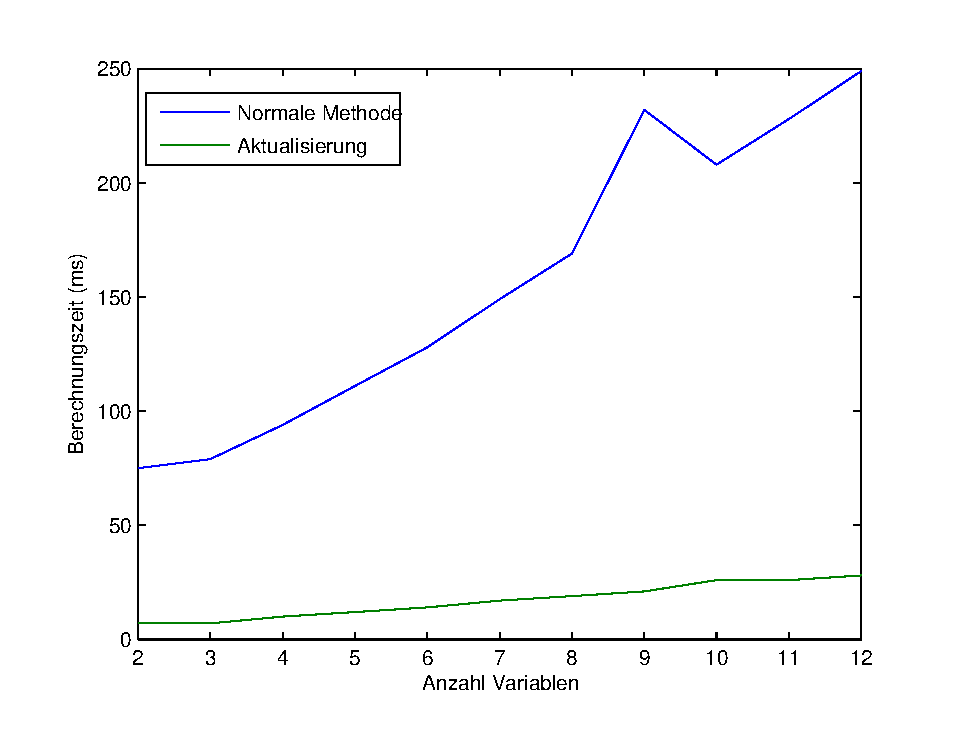
\includegraphics[width=0.6\textwidth]{figures/multi_reg_vars_2500_obs_act}
    }
    \subfloat[][Unterschied zwischen direkter Berechnung und Aktualisierung mit zufälligen Daten]{
      \label{fig:analysis:mul_reg_rand_act}
      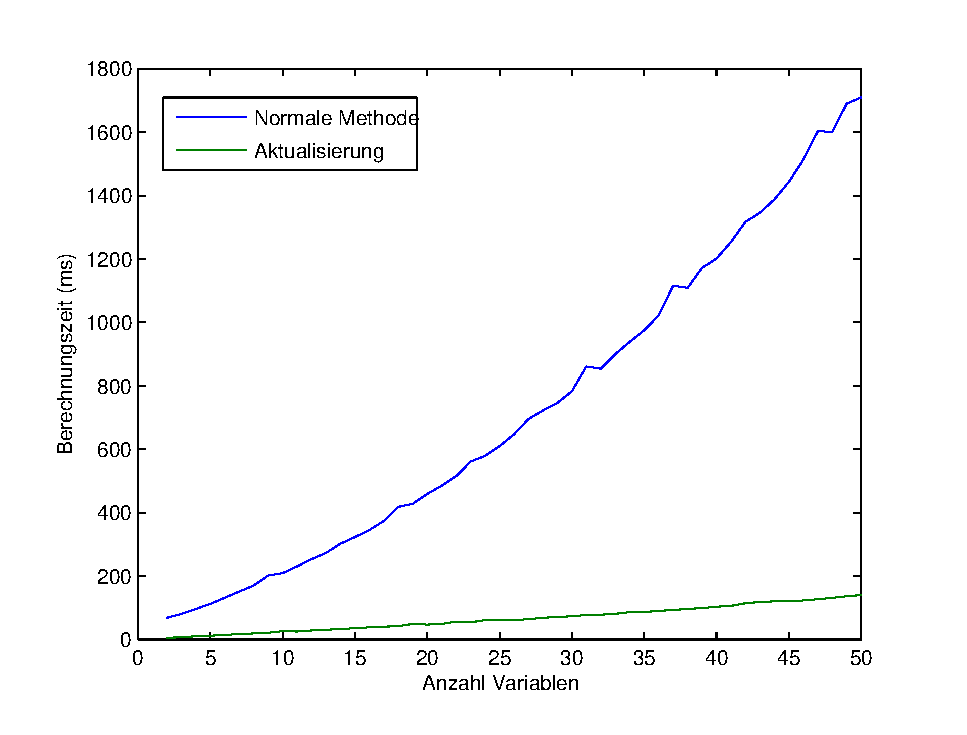
\includegraphics[width=0.6\textwidth]{figures/multi_reg_vars_2500_obs_act_rand}
    }
  \end{narrow}
  \caption{Ergebnisse der Leistungsanalyse.}
  \label{fig:analysis}
\end{figure}

% TODO: Leistungsanalyse Korrelationsfunktion ...

Für die Regression werden wir jeweils 

%%% Local Variables: 
%%% mode: latex
%%% TeX-master: "report"
%%% End: 
